\documentclass[a4paper,oneside,12pt]{article} % jednostrano: promijeniti twoside u oneside
\usepackage[utf8]{inputenc} 
\usepackage[croatian]{babel}
\usepackage[pdftex]{hyperref} % ukoliko se koristi XeLaTeX onda je \usepackage[xetex]{hyperref}
%\usepackage{txfonts} % times new roman 
\usepackage[pdftex]{graphicx} 
\usepackage{cleveref}
\usepackage{amsmath}
\usepackage{amsfonts}
\usepackage{amssymb}
\usepackage{amsthm}
\newtheorem{lmdef}{Definicija}
\newtheorem{lmth}{Teorem}
\newtheorem{lmlem}{Lema}
\newtheorem{lmrez}{Rezultat}
\newtheorem{lmnap}{Napomena}


\pagestyle{headings}
\title{Valiantovo poboljšanje CYK algoritma}
\author{Luka Mikec}

\begin{document}
    \maketitle

    \section{Uvod}
    Prepoznavanje, ili parsiranje u užem smislu,\footnote{Pod parsiranjem se (u širem smislu) nekad
        podrazumijeva gradnja sintaksnog stabla. Ovdje nas zanima samo prepoznavanje. } 
        je dobro istražen problem teorijskog računarstva.
    Za danu formalnu gramatiku $G = (V, T, P, S)$ 
        te relaciju izvodivosti
        $\xrightarrow{*}\ \subseteq (V \cup T)^* \times (V \cup T)^*$,
        problem prepoznavanja je određivanje vrijedi li $S \xrightarrow{*} w$
        za danu riječ $w \in (V \cup T)^*$.

   Povijesno, razvoj algoritama za prepoznavanje je fokusiran na kontekstno neovisne jezike.
   Širi fokus vodi u inherentnu sporost ili teorijske probleme (neizračunljivost),
       a uz to se gubi veza s lingvističkim pojmom gramatike.
   Uži fokus je međutim čest. Većina modernih algoritama za prepoznavanje radi s
       raznim pravim podskupima konteksno neovisnih jezika.
   Uži fokus omogućava linearne ili skoro-linearne algoritme.
   
   U nastavku pod prezponavanjem podrazumijevamo prepoznavanje konteksno neovisnih jezika,
       dakle nećemo pojednostavniti problem.
   
   Mjera složenosti prepoznavanja je broj simbola riječi na ulazu.
   Gramatika (odnosno njena veličina) se zanemaruje zbog pretpostavke da 
       ćemo gramatiku obraditi najviše jednom,
       a testirati prepoznavanje neograničeno mnogo puta.
   Ta pretpostvka ne mora vrijediti u nekim egzozičnijim domenama,
   Ako bi nas utjecaj veličine gramatike zanimao za algoritam o kojem je riječ u ovom radu, 
       unutar \emph{velikog $O$} bismo trebali dodati $|G|^2$ u sve mjere složenosti.
   Dakle, u nastavku trajanje procesiranja gramatike smatramo konstantom.
   U praktičnoj primjeni prepoznavanja koriste se algoritmi čija je gornja granica složenosti $O(n^3)$.
   
   Cilj ovog rada je predstaviti asimptotski najefikasniji poznat algoritam.
   Radi se o Valiantovom proširenju CYK algoritma (u nastavku: Valiantovom algoritmu).
   Složenost Valiantovog algoritma svodi se na složenost korištenog algoritma za množenje matrica.
   Iz toga slijedi da je problem prepoznavanja,
       zbog Valiantov algoritma,
       barem $O(n^{2.3728639})$, što je složenost trenutno najbržeg poznatog 
       algoritma za množenje dvije matrice.
    
    
   \section{Valiantov algoritam}
   \subsection{Obrada gramatike}
    
   U prvom dijelu algoritma iz dane gramatike $G = (V, T, P, S)$ generiramo gramatiku
       $G' = (V', T, P', S')$ sa sljedećim svojstvima:
   \begin{itemize}
       \item $S \xrightarrow{*} w$ akko $S' \xrightarrow{*} w$, za $w \in T^*$.
       \item $P'$ sadrži samo produkcije oblika $A \to BC$ i $A \to b$, 
           za proizvoljne neterminalne simbole $A$, $B$ i $C$,
           i također proizvoljan terminalni simbol $b$.
    \end{itemize}
    Dakle, relacija $\xrightarrow{*}$ se mora podudarati samo za riječi
        u jeziku terminalnih simbola izvorne gramatike.
    Ovisno o definiciji kojoj se priklonimo, kaže se da je $G'$ 
        u Chomskyjevoj normalnoj formi ili njenoj varijanti.
        
    Postupak generiranja $G'$ iz $G$ je standardan te ga samo ukratko opisujemo.
    Detalji algoritma se mogu pogledati u implementaciji \verb|grammar::to_cfg()| metode
        u datoteci \emph{grammar.cpp}.
    \begin{enumerate}
        \item Radni skup produkcija inicijalizira se s $P$.
        \item Za svaki završni simbol $t \in T$ gradimo novi nezavršni znak $[t] \in t^*$,
            te dodajemo produkciju $[t] \to t$ u $P'$ u $V'$.
            U produkcijama radnog skupa mijenjamo $t$ s $[t]$.
        \item Pretragom u dubinu skupa $P$ 
            tražimo sve lance oblika $A_0 \to A_1,\ A_1 \to A_2,\ A_2 \to ...$ gdje je $A_i \in V$.
            Nakon što smo pronašli sve takve lance,
                brišemo produkcije iz lanaca te 
                dodajemo produkciju $A_i \to BW$ za svaku produkciju $A_j \to BW$,
                gdje je $B \in V,\ W \in V^* \setminus \{ \epsilon \} $
                i vrijedi $i < j$.
        \item Neka je dana produkcija $A \to A_1...A_{2n - 1}$.
            Zbog prethodnog koraka vrijedi $n > 1$. 
            \begin{itemize}
                \item Ako $n = 1$:
                    brišemo tu produkciju i dodajemo $A \to XA_3$ te
                    $X \to A_1A_2$.
                \item Ako $n > 2$:
                Brišemo tu produkciju i dodajemo $A \to XY$,
                    $X \to A_1A_2$ te $Y \to A_3...A_{2n-1}$.
                Rekurzivno ponavljamo ovu točku na $Y$.
            \end{itemize}
        \item Neka je dana produkcija $A \to A_1...A_{2n}$ za $n > 1$.
        \begin{itemize}
            \item Ako $n = 2$:
            brišemo tu produkciju i dodajemo $A \to XY$,
            $X \to A_1A_2$ te $Y \to A_1A_2$.
            \item Ako $n > 2$:
            Brišemo tu produkciju i dodajemo $A \to XY$,
            $X \to A_1A_2$ te $Y \to A_3...A_{2n}$.
            Rekurzivno ponavljamo ovu točku na $Y$.
        \end{itemize}
    \end{enumerate}
   
    U koracima 3-5 broj produkcija gramatike se neće povećati više nego kvadratno,
        tj. $|P'| \leq |P|^2$.
        
    \subsection{Klauzule i matrica parsiranja}
    Pretpostavljamo da je dana obrađena gramatika $G = (V, T, P, S)$ i riječ $w \in T^*$.
    
    Sljedeći pojmovi nam trebaju kako bismo mogli koristiti
        neke uobičajene algebarske operacije u nastavku algoritma.
    
    \begin{lmdef}
        Klauzula je (možda prazan) podskup skupa $V$. 
        Skup svih klauzula označavamo s $K$.
    \end{lmdef}
    Očito vrijedi $K = 2^V$. 
    Može biti korisno identificirati klauzulu s vektorom binarnih znamenki
        $b_k = (b_1, b_2, ..., b_{|V|})$.
    Pojam klauzule preuzimamo iz propozicijske logike,
        jer želimo da neformalna interpretacija klauzule $k = \{k_1, ..., k_n\}$
        bude $k_1$ ili $k_2$ ili ... ili $k_n$,
        kao što je slučaj s klauzulama konjunktivne normalne forme.
    
    \begin{lmdef}
        Definiramo algebarsku strukturu $(K, +, *)$ na sljedeći način.
        \begin{itemize}
            \item $K$ je skup klauzula.
            \item Za $k_1, k_2\in K$ definiramo:
            \[ k_1 + k_2 := k_1 \cup k_2. \]
            \item Za $k_1, k_2\in K$ definiramo:
            \[ k_1 * k_2 := \{ A\ |\ (A \to XY) \in P,\ X \in k_1,\ Y \in k_2  \}. \]
        \end{itemize}
    \end{lmdef}
    
    \begin{lmth}
        Struktura $(K, +)$ je komutativni monoid s neutralnim elementom $\epsilon$.
        Vrijedi distributivnost $*$ preko $+$.
    \end{lmth}
    \begin{proof}
        Prva tvrdnja slijedi izravno iz definicije operacije zbrajanja.
        Za drugu tvrdnju je dovoljno raspisati $k_1*(k_2 + k_3)$
            i $(k_2 + k_3) * k1$, te koristiti definiciju unije
            i De Morganova pravila.
    \end{proof}
    
    Sad možemo definirati glavnu podatkovnu strukturu Valiantovog algoritma.
    Spomenimo da sva indeksiranja, 
        ako nije drugačije navedeno,
        počinju od $0$.
    
    \begin{lmdef}
        Osnovna matrica parsiranja $M'$ je $(|w| + 1) \times (|w| + 1)$ 
            matrica nad $K$ za koju vrijedi:
        \begin{itemize}
            \item $M'_{i, i+1} = \{A | A \to w_i\}$.
            \item $M'_{r, c} = \emptyset$ za $c \neq r + 1$.
        \end{itemize}
        Matrica parsiranja $M$ je 
            $2^{\lceil \log_2 (|w| + 1) \rceil } \times 2^{\lceil \log_2 (|w| + 1) \rceil }$
            matrica nad $K$ čiji je gornji desni $(|w| + 1) \times (|w| + 1)$ kut jednak $M'$
            a preostale ćelije jednake $\emptyset$.
    \end{lmdef}
    
    Matrice se obično definiraju nad poljem.
    No, $K$ nije polje. 
    Ipak, $K$ dopušta množenje i pribrajanje, što omogućava korištenje
        uobičajenog $O(n^3)$ algoritma za množenje matrica.
    Neki drugi algoritmi za množenje matrica nad poljima
        neće producirati ekvivalentan rezultat 
        kao uobičajeni $O(n^3)$ algoritam.
    Stoga te druge algoritme u ovom kontekstu ni ne smatramo
        algoritmima za množenje matrica.
    
    \begin{lmnap}
        Neka je $M$ matrica parsiranja, te $R = M^2$.
        
        Neka postoji produkcija $A \to BC$, te vrijedi $A \in M_{i,\_}$ i $B \in M_{\_, j}$
            za $i < j$.
        Tada vrijedi $A*B = C \in R_{i,j}$.
        Dakle, množenjem matrice parsiranja zapravo gradimo sva moguća
            stabla parsiranja, i to na \emph{bottom-up} način 
            od donjeg-lijevog prema gornjem-desnom kutu matrice.
            
        
        Neka je $M^{(0)}$ matrica praznih klauzula (praznih skupova) dimenzija kao $M$,
        te $M^{(1)} := M$.
        Ako za $n > 1$ označimo 
        \[
            M ^{(n)} = \bigcup_{n = \sum_{i = 0}^{k} n_i} \left( \prod_{j = 0}^n M^{(n_j)} \right)
        \]
        onda će gornji desni $(|w| + 1) \times (|w| + 1)$ kut matrice $M^{(k)}$ na poziciji 
            $(0, k)$ imati klauzulu koja sadrži točno sve nezavršne znakove
            koji produciraju $k$-prefiks riječi $w$.
        Za $k = |w|$ stoga možemo očitati sadrži li klauzula početni nezavršni znak
            $S$ ili ne.    
            
        Očito je izravan račun ove matrice neefikasan. 
        Izvorni algoritam koji slijedi ovaj pristup (Cocke–Younger–Kasami)
            nudi $O(n^3)$ izračun,
            no Valiantov pristup možda nudi i $O(n^2)$ 
            (ovisno o neriješenom problemu složenosti množenja matrica).
    \end{lmnap}
    
    
    \subsection{Zatvorenje (pod)matrica parsiranja}
    
    Temeljni je doprinos Valiantovog algoritma efikasan izračun 
        problema iz upravo dane napomene.
    Primijetimo da je izračun $M^{(|W|)}$ ekvivalentan izračunu
        $M^{(\infty)}$ (tranzitivnom zatvorenju s obzirom na potenciranje).
    Za zatvorenje ćemo koristiti kraću oznaku $M'$.
    
    Sada definiramo nekoliko ključnih operacija u algoritmu.
    Koristit ćemo notaciju $A(i:j,\ k:l)$ za označiti
        podmatricu matrice $A$ koja sadrži retke od $i$ (uključno) do $j$ (isključno)
        te stupce od $k$ (uključno) do $l$ (isključno).
        
    \begin{lmdef}
        Definiramo operacije: \verb|zatvorenje|, \verb|lema|, \verb|p2|, \verb|p3| i \verb|p4|.
        S $m$ ćemo označiti broj redaka, a s $n$ broj stupaca, podmatrice koja je parametar operaciji.
        Pridruživanje $:=$ je po vrijednosti (duboko kopiranje), a $=$ po referenci.
        Proslijeđivanje argumenata je uvijek po referenci.
        
        \verb|zatvorenje| $\leftarrow$ podmatrica $M$ \\
        Ako je $m == 1$, zaustavi.\\
        Izračunaj \verb|zatvorenje| $M(0:\frac{m}{2},\ 0:\frac{m}{2})$. \\
        Izračunaj \verb|zatvorenje| $M(\frac{m}{2}:m,\ \frac{m}{2}:m)$. \\
        Izračunaj \verb|p2| $M$. \\
        
        \verb|p2| $\leftarrow$ podmatrica $M$ \\
        Ako je $m < 4$, zaustavi.\\
        Izračunaj \verb|p2| $M(\frac{m}{4}:\frac{3m}{4},\ \frac{m}{4}:\frac{3m}{4})$. \\
        Izračunaj \verb|p3| $M(0:\frac{3m}{4},\ 0:\frac{3m}{4})$. \\
        Izračunaj \verb|p3| $M(\frac{m}{4}:m,\ \frac{m}{4}:m)$. \\
        Izračunaj \verb|p4| $M$. \\
        
        \verb|p3| $\leftarrow$ podmatrica $M$ \\
        Ako je $m < 3$, zaustavi.\\
        Izračunaj \verb|lema| $M$, $\frac{2m}{3}$. \\
        
        \verb|p4| $\leftarrow$ podmatrica $M$ \\
        Ako je $m < 4$, zaustavi.\\
        Izračunaj \verb|lema| $M$, $\frac{3m}{4}$. \\
        
        \verb|lema| $\leftarrow$ podmatrica $M$, cijeli broj $r$ \\
        Ako je $n = 1$, zaustavi. \\
        $c = M(0:n-r,\ n-r:r) * M(n-r:r,\ r:n)$. \\
        $M' := M$. \\
        $M'(0:n-r\ r:n)\ \mathrel{+}=\ c$. \\
        $M'' = M'.$\verb|ukloni_retke|$(n-r, r).$\verb|ukloni_stupce|$(n-r, r)$. \\
        Izračunaj \verb|zatvorenje| $M''$. \\
        $M(0:n-r,\ r:n)\ \mathrel{+}=\ M''(0:n-r,\ n-r:2(n-r))$.
        
    \end{lmdef}
    
    Riječima, operacija \verb|zatvorenje| prvo izračuna 
        zatvorenja gornje lijeve podmatrice, te donje desne podmatrice.
    Potom mora izračunati gornji desni ``ostatak''
        što rekurzivno izvodi procedura \verb|p2|.
    Procedura \verb|p2| prvo izračuna zatvorenje ``sredine'',
        pa potom gornje lijeve i donje desne podmatrice uz pomoć procedure \verb|lema|. 
    Na kraju se opet uz pomoć procedure \verb|lema| ti rezultati spajaju.
       
    
    \subsection{Množenje Boolovih matrica}
    
    U ovom trenutku je najbrži poznati algoritam za množenje Boolovih matrica
        ekvivalentan najbržem poznatom algoritmu za množenje matrica nad proizvoljnim poljem.
    U budućnosti će se to možda promijeniti.
    
    Valiantov algoritam, kakav je do sada prezentiran, ima složenost $O(n^3)$.
    Ta složenost potječe iz složenosti korištenog algoritma za množenje matrica.
    Taj algoritam ne možemo zamijeniti asimptotski bržim algoritmima jer oni pretpostavljaju
        bogatije algebarske strukture od ranije definirane strukture $K$.
    No, problem množenja matrica nad $K$ svodiv je na množenje Boolovih matrica
        uz asimptotski zanemarivo malo više posla. 
    Boolove matrice dopuštaju upotrebu bržih algoritama za množenje matrica.
    
    Postupak je sljedeći. 
    Za matrice $A$ i $B$ izradimo $2|V|$ pomoćnih Boolovih matrica 
        u koje za svaki nezavršni simbol zapišemo javlja li se u odgovarajućoj ćeliji
        osnovnih matrica ili ne ($1$ za odgovaranje, $0$ inače).
       
    Potom izradimo $|V|^2$ pomoćnih Boolovih matrica u koje spremimo rezultate
        množenja svih pomoćnih matrica za $A$ sa svim pomoćnim matricama za $B$.
    
    Na taj način zapravo saznajemo za svaku ćeliju rješenja imamo 
        li u njoj umnožak svake moguće kombinacije nezavršnih simbola.
    U $O(n^2)$ možemo ``poravnati'' spomenutih $|V|^2$ matrica,
        jer moramo proći svakom ćelijom, a faktor gramatike po ranijem običaju ignoriramo.
    Kako su sama množenja matrica barem $O(n^2)$, 
        ispada da je cijeli postupak asimptotski dominiran složenošću samog množenja matrica.
    U ovom trenutku je najbrži poznat takav algoritam 
        inačica Coppersmith–Winogradovog algoritma sa složenošću $O(n^{2.3728639})$.
        
    \section{Implementacija}
    
    Algoritam je u cijelosti implementiran i dostupan na adresi
        \url{https://github.com/luka-mikec/valiant-parsing}.
    Implementirani su i neki pomoćni alati poput učitavanja proizvoljne gramatike
        te generiranja jezika za danu gramatiku.
        
    Iako postoje implementacije podijeli-pa-vladaj i CYK-baziranih algoritama,
        ovo je možda prva javna implementacija izvornog Valiantovog algoritma.
    Ova implementacija ne nudi asimptotski najbrže moguće (poznato) parsiranje 
        jer ne koristi spomenuti Coppersmith–Winogradov	
        algoritam već obično množenje matrica. 
    Drugi algoritmi se mogu koristiti postavljanjem statičke varijable
        \verb|matrix_view<bool>::mul_op| na željeni algoritam.
        
    \begin{figure}
        \centering
        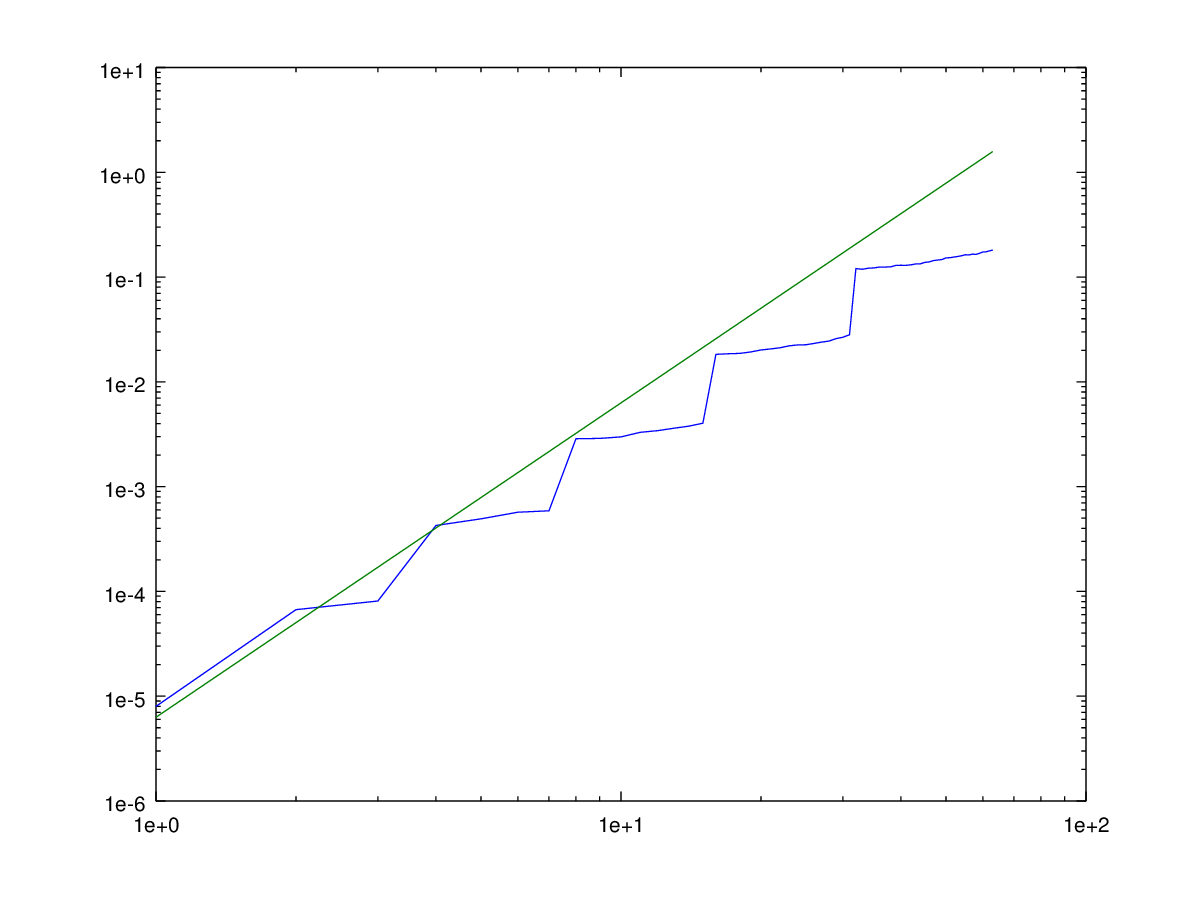
\includegraphics[scale=0.5]{graf.png}
        \caption{\small Trajanje algoritma na riječima $|w| = 1$ do $w = 63$, usporedba s $n^3$. 
            Graf je log-log.}
    \end{figure}
        
    Detalji implementacije i korištenja mogu se pronaći na adresi
        \url{https://github.com/luka-mikec/valiant-parsing}.
        
    
    \section{Literatura}

    \noindent Valiant, Leslie G. ``General context-free recognition in less than cubic time.'' 
    \emph{Journal of computer and system sciences} 10.2 (1975): 308-315.

\end{document}
